\documentclass{article}
\usepackage[UTF8]{ctex}  %加载包,因为我们在用中文写文档,所以必须加载这个包,否则不支持中文
\usepackage{multicol}  %加载包
\usepackage[top=1in, bottom=1in, left=1.25in, right=1.25in]{geometry}  %加载包
\usepackage{lscape}
\usepackage[colorlinks,linkcolor=blue]{hyperref}
\usepackage{amsmath}
\usepackage{tikz}
\usepackage{pgfplots}
\author{VincentZhang}  % 作者
\date{2019.7.30}  %定义时间
\title{流体力学}  %文档标题
\begin{document}

\maketitle
前言,这篇文章是2007年Siggraph的课程文档(Course Note),从头到底很详细的讲解了怎么用计算机模拟流体(烟和水等等)。
原文地址: \url{https://www.cs.ubc.ca/~rbridson/fluidsimulation/fluids_notes.pdf}

\section{第一章 流体力学公式}
流体力学中最重要的公式是Navier-Stokes 公式:
\begin{equation}
\frac{\partial{\vec{u}}}{\partial{t}}+\vec{u}\cdot \nabla{\vec{u}}+\frac{1}{\rho}\nabla{p}=\vec{g}+\nu\nabla\cdot\nabla\vec{u} \label{momentumequation}
\end{equation}
\begin{equation}
\nabla\cdot\vec{u}=0 \label{incompressibilitycondition}
\end{equation}

\subsection{符号含义}
其中$\vec{u}$是流体的速度。\par
$\rho$是流体的密度,大家都熟悉,如果是水的话,其值为$1000kg/m^3$. 如果是空气的话,其值为$1.3kg/m^3。$\par
$p$是压力,流体对内对外的压力。\par
$vec{g}$是大家都熟悉的重力加速度,一般性就是中学书上的值$(0,-9.81,0)m/s^2$。 从这个向量表示也行,我们这里y轴像上。x- 轴,y- 轴是水平的。$\vec{g}$有时候大家也会叫他"体作用力"\par
$\nu$是“静态粘度”。顾名思义,这个参数表达的是流体有多粘稠。像糖浆这样的流体这个值很高,像酒精这样的流体这个值很低。学术点说,这个参数反映了流体抗拒形变的程度。一个极端的例子是沥青,网上不是有个段子,有个科学家等了一辈子想看一颗沥青掉下来的过程,最后到死都没有实现。另一个更加极端的例子是玻璃,玻璃其实也是一种流体,有很多几百年老教堂的玻璃窗,下面比上面厚,这就是流体流动的结果,但是大家懂的,要观察玻璃滴下来,估计这个老教授要等到宇宙尽头了。
\subsection{动量方程}
Navier-Stokes里的第一条方程(\ref{momentumequation}),其实是一条向量方程,另有一个名字叫做"动量方程",所以看这条方程的时候,千万要注意变量上面的箭头。其实这个方程就是变形的牛二方程$\vec{F}=m\vec{a}$。 这个方程告诉了我们流体在各种作用力之下是怎么运动的。显然这条方程比较复杂,这一节将把这个方程拆开一项项给大家讲解。后一章节,我们将介绍(\ref{incompressibilitycondition}),这个方程叫做“不可压缩条件”。\par
现在先假设我们用粒子系统去模拟流体(实际上后面的章节有讲怎么具体去模拟,这里作此假设只是进行理论推导方便)。每一个粒子,都可以被理解为一个小小的"分子团",这个“分子团”的质量为m,体积为V(这点很重要,注意我们不是用单个分子去模拟粒子,而是一个小小的分子团!),速度为$\vec{u}$。 根据牛二定理,只要我们知道了这个“分子团”上面的所有的力,根据$\vec{F}=m\vec{a}$ 我们就能知道这个“分子团”的加速度了。其中加速度,我们用这种奇怪的方式定义:\begin{equation}
\vec{a}\equiv\frac{D\vec{u}}{Dt}
\end{equation}
这里面大写的D,叫做物质导数或者叫随体导数。如果你能打开这个链接的话,Wiki上有很好的解释\url{https://en.wikipedia.org/wiki/Material_derivative}。 百度百科上的解释是这样的:\url{https://baike.baidu.com/item/%E9%9A%8F%E4%BD%93%E5%AF%BC%E6%95%B0} \par
简单来说,随体导数是流体力学中的术语。研究的是流体在某点的力学状态时,常考虑这个点周围很小范围内的物质(也就是我们说的“分子团”)随时间变化的变化率。比如这个”分子团“的体积随时间的变化率,再如”分子团“组成的平面随着时间的变化率等等。\par
用随体导数改写的牛二定理如下:
\begin{equation}
m\frac{D\vec{u}}{Dt}=\vec{F}
\end{equation}
OK,接下来我们就来看下粒子上受到了哪些力。最简单的当然是重力:$m\vec{g}$。但是这肯定不是唯一的力,其他粒子也对这个粒子有作用力。\par
第一种来自其他粒子的力,是压力。高压区域的粒子持续不断的给低压区域的粒子施加压力,比如正是由于有心脏不断跳动,向血液施加压力,血液才能流遍全身)。请注意,我们这里的压力,考虑的是合力,具体这个力是从哪个粒子来的并不重要。大家都挤过地铁吧,想象我们现在站在一节塞满了人的地铁车厢里面,真的是塞得满满当当的。这时候突然你的左手边开门了,瞬间你左边的人都走光了,这时候你会受什么力呢?当然是从右向左的力啦,你右边的人也想下车但是被你挡住了啊,只能推你!\par
具体到流体的粒子,假设流体受到的总压力分布为p(注意,这是一个矢量场,不同的位置有不同的压力值), 那么在某点的压强是多少呢?在该点对压力取梯度就可以了,也就是$-\nabla p$,那么我们这个”分子团“上面受到的总压力是多少呢?理论上讲是对$-\nabla p$在整个粒子团的表面取积分,这么做很难,所以我们一般就简简单单乘以体积进行近似。结果粒子上的总压力为:$-V\nabla p$。负号表示这个力是粒子团抵抗外界压力的力,压力的存在主要是因为粒子团想要维持自己的体积,这一点在后续”不可压缩条件“这部分会有更详细解释。\ par
第二种来自其他粒子的力为粘性力,粘性力的主要作用是抵制流体的形变。粘性力存在的原因应该是流体内部的摩擦力。其效果是让瘤体内的粒子(分子团)的速度尽量跟周围粒子的平均速度一样,也就是说,尽量降低流体内部的速度差。如果你做过图像处理,或者了解热传导方程或扩散方程,那就应该能知道,数学上描述某一个特定点的数量与周围点平均值的差距是拉普拉斯算子$\nabla\cdot\nabla$,这个量在这里是速度,因此这个部分是$\nabla\cdot\nabla\vec{u}$。下一节会更详细解释拉普拉斯算子,别着急。更压力的情况差不多的是,粘性力也需要对整个粒子进行积分。因此我们得到了:$V\nu\nabla\cdot\nabla\vec{u}$,其中$\nu$是流体的动态粘性系数,由很多因素决定,常见液体的粘度随温度升高而减小,常见气体的粘度随温度升高而增大。\par
总结下,一个粒子团总共受到三种力,重力、压力、粘性力。把上面的所有项都放在一起,我们就得到了:
\begin{equation}
m\frac{D\vec{u}}{Dt}=m\vec{g}-V\nabla{p}+V\nu\nabla\cdot\nabla\vec{u}
\end{equation}
等式两边除以体积,得到:
\begin{equation}
\rho\frac{D\vec{u}}{Dt}=\rho\vec{g}-\nabla{p}+\nu\nabla\cdot\nabla\vec{u} \label{momentumequation_1st}
\end{equation}
其中$\rho$为流体密度。

\fbox{
\parbox{\textwidth}{
简单解释下拉普拉斯算子$\nabla\cdot\nabla$,详细的解释请参见多维微积分教材 \\
拉普拉斯算子,记作$\nabla\cdot\nabla$、$\nabla^2$ 或者$\Delta$,为梯度的散度。顾名思义,他的含义是先对函数f(一般至少是二维函数)做梯度$\nabla{f}$, 再对这个梯度函数做散度$\nabla\cdot\nabla{f}$。\\
这么说还是很抽象,我们来考虑下二维离散的图片,在某一点的拉普拉斯算子(四联通)可以这样定义:
\begin{equation}
\nabla\cdot\nabla{f}=[f(x+1,y)+f(x-1,y)+f(x,y+1)+f(x,y-1)]-4f(x,y) \label{laplacian}
\end{equation}
如果用卷积核的方式来表示,就是:
$$
\left[
\begin{matrix}
0 & -1 & 0 \\
-1 & 4 & -1 \\
0 & -1 & 0
\end{matrix}
\right]
$$
从(\ref{laplacian})可以很明显看出,拉普拉斯算子衡量的是一个点的数值偏离周围点数值平均值的程度。在图像处理上,主要用来做边缘检测。
}
}

在式(\ref{momentumequation_1st})的两边除以$\rho$,得到下式:
\begin{equation}
\frac{D\vec{u}}{Dt}=\vec{g}-\frac{1}{\rho}\nabla{p}+\frac{\nu}{\rho}\nabla\cdot\nabla\vec{u}
\end{equation}
其中的$\frac{\nu}{\rho}$叫做静态粘性系数,记作$\nu$ 因为除了液体的密度,所以显然密度越大的流体,这个值越高。代入上式,再整理下得到:
\begin{equation}
\frac{D\vec{u}}{Dt}+\frac{1}{\rho}\nabla{p}=\vec{g}+\nu\nabla\cdot\nabla\vec{u}
\end{equation}

\subsection{拉格朗日视角与欧拉视角}
当需要考虑可变性的连续体运动的时候(流体或者那种会变形的固体,比如布料等等。我们这篇文章讲的是流体,后文没有特别注明的情况下都用流体去考虑),有两种视角,拉格朗日视角和欧拉视角。\par
拉格朗日视角的观点基本上就是让观察者变身成流体里面一个"分子团",假设你就是这个"分子团",那么你的位置$\vec{x}$、速度$\vec{u}$会是什么?从这个角度去考虑流体里的量的变化的方法,叫做拉格朗日视角。\par
欧拉视角,基本上主要考虑空间中固定点的量,因为这个点是固定的其位置不会变化,考虑流经这个点的其他量比如速度$\vec{x}$、 密度$\rho$,温度等等的变化。 比如,如果正好一股暖流从这个固定点经过,如果我们考虑这点的温度,会看到它不断上升。但是如果用拉格朗日视角一个个粒子去看,其实整个流体里面没有一个粒子的温度有变化。\par
一个更有趣的粒子是天气预报,拉格朗日视角其实就像是个探空气球,跟着风到处飞。欧拉视角就像是那些放在地面上,测吹过的空气的温度湿度的百叶箱。\par
从数值模拟的角度,拉格朗日视角其实就是做一个粒子系统(可能用一个网格连接起来),欧拉视角则是一个在空间中不随流体运动的固定格子,考虑的是每个格点上的物理量。\par
这么看起来,拉格朗日视角似乎更加好理解也更简单,那为什么我们还需要引入欧拉视角呢?主要有如下原因:
\begin{itemize}
\item 用欧拉视角,比较有助于理论分析压力梯度和粘性力。
\item 由于流体形状多变,在一个固定网格上对各种量进行差分等数值模拟也会相对比较简单。
\end{itemize}
把这两种视角联系起来的关键是物质导数。让我们先从拉格朗日视角开始描述下物质导数:有一个“分子团”,它的位置是$\vec{x}$,速度是$\vec{u}$。 假设这个粒子拥有某个物理量q(可能是压力,可能是密度,可能是温度,这里的讨论不限于具体是哪个物理量,只是做一个统一的理论分析)。这样函数$q(t,\vec{x})$指的就是在t时刻,经过$\vec{x}$的物理量q的值,如果是一个固定点$\vec{x}$的话,显然,这就是个欧拉视角下的变量,其变化率(即该物理量随时间变化的速率)是什么呢?用链式法则算一下:
\begin{equation}
\begin{aligned}
\frac{d}{dt}q(t,\vec{x})&=\frac{\partial{q}}{\partial{t}}+\nabla{q}\cdot\frac{d\vec{x}}{dt} \\
&=\frac{\partial{q}}{\partial{t}}+\nabla{q}\cdot\vec{u} \\
&\equiv{\frac{Dq}{Dt}}
\end{aligned}
\end{equation}
可以看到物质导数有两项,第一项$\frac{\partial{q}}{\partial{t}}$,指的该物理量在$\vec{x}$这点随时间变化的变化率。第二项$\nabla{q}\cdot\vec{u}$ 指是该物理量随着流体运动的变化率。\par
注意物质导数是向量,当然我们可以把它在3d的坐标系中展开(可以想象一下,在四维空间,流体是怎样的呢?五维、六维以至于无穷维呢?),注意到$\nabla{q}=(\frac{\partial{q}}{\partial{x}},\frac{\partial{q}}{\partial{y}},\frac{\partial{q}}{\partial{z}})$,将它与速度向量$\vec{u}=(u,v,w)$做点积可以得到:
\begin{equation}
\frac{Dq}{Dt}=\frac{\partial{q}}{\partial{t}}
                +u\frac{\partial{q}}{\partial{x}}
                +v\frac{\partial{q}}{\partial{y}}
                +w\frac{\partial{q}}{\partial{z}} \label{materialderivative}
\end{equation}
显然在2D空间中,上式最后一项$w\frac{\partial{q}}{\partial{z}}$ 为零,可以去掉。\par
式(\ref{materialderivative})表示的某个物理量随着"分子团"在速度场中$\vec{u}$中运动的情况,这种运动叫做对流。如果某个物理量,它在拉格朗日视角下没有任何变化(比如假设外界温度不变的情况下,温度在空气中随着风而传播的过程),那么我们可以得到对流方程:
\begin{equation}
\begin{aligned}
\frac{Dq}{Dt}\equiv{0} \\
i.e. \frac{\partial{q}}{\partial{t}}+\nabla{q}\cdot\vec{u}=0
\end{aligned}
\end{equation}

\subsection{一个例子}
写一堆公式都不如直接来个例子让人好理解,所以我们这里先举个温度的例子。因为这个具体的例子是用的温度这个物理量,所以这里不用q而用T。假设这个温度场是这样的:
\begin{equation}
T(x)=10x
\end{equation}
也就是说,越在右边,温度越高,左边温度低。在坐标原点,温度为零,在图的右边$x=100$ 的地方,温度为100。假设有一个稳定的速度为c的风向右吹,这样的话,流速的分布是这样的:
\begin{equation}
\vec{u}=c
\end{equation}
为简单起见,假设空气中每个粒子本身的温度不发生变化,只是移动。就像上章说过的,这种情况下,用拉格朗日视角看,随体导数为零。
\begin{equation}
\frac{DT}{Dt}=0
\end{equation}
展开可以得到:
\begin{equation}
\begin{aligned}
\frac{\partial{T}}{\partial{t}}+\nabla{T}\cdot\vec{u}=0 \\
\frac{\partial{T}}{\partial{t}}+10\cdot{c}=0 \\
\Rightarrow \frac{\partial{T}}{\partial{t}}=-10c \label{example}
\end{aligned}
\end{equation}
从式(\ref{example})可以看到,在空间中一个固定点,温度的变化率是-10c。如果风速降低到c=0,那么整个流体都不发生任何变化。如果向右吹的速度c=1,在固定点的温度变化率为-10度每秒。如果风吹的更大一点c=20,那么在每个固定点的温度变化率为-20度每秒。可以看到即使拉格朗日视角下,温度变化为零,欧拉视角下温度仍然在流体速度的作用下不断变化。
\subsection{对流向量}
初学者经常困惑的一点是在向量的情况下,随体导数的意义,例如颜色RGB的随体导数,或者更明确的说,速度向量场$\vec{u}$的随体导数是什么含义。最简单的答案:把每个分量单独处理。让我们把颜色向量$\vec{C}=(R,G,B)$,那么其随体导数为:
\begin{equation}
\frac{D\vec{C}}{Dt}=\begin{bmatrix}
    DR/Dt \\
    DG/Dt \\
    DB/Dt
\end{bmatrix}=\begin{bmatrix}
\partial{R}/\partial{t}+\vec{u}\cdot\nabla{R} \\
\partial{G}/\partial{t}+\vec{u}\cdot\nabla{G} \\
\partial{B}/\partial{t}+\vec{u}\cdot\nabla{B}
\end{bmatrix}=\frac{\partial{\vec{C}}}{\partial{t}}+\vec{u}\cdot\nabla\vec{C} \label{advect_vector}
\end{equation}
接下来,我们都速度进行一下同样的操作,基本上没什么大区别,就把上两次出现的$\vec{C}$用$\vec{u}$来代替就行了。用$\vec{u}=(u,v,w)$带入,得到:
\begin{equation}
\frac{D\vec{u}}{Dt}=\begin{bmatrix}
Du/Dt \\
Dv/Dt \\
Dw/Dt
\end{bmatrix}=\begin{bmatrix}
\partial{u}/\partial{t} + \vec{u}\cdot\nabla{u} \\
\partial{v}/\partial{t} + \vec{u}\cdot\nabla{v} \\
\partial{w}/\partial{t} + \vec{u}\cdot\nabla{w}
\end{bmatrix}=\frac{\partial{\vec{u}}}{\partial{t}}+\vec{u}\cdot\nabla{\vec{u}}
\end{equation}
当然,我们可以进一步展开右边的梯度项得到下式:
\begin{equation}
\frac{D\vec{u}}{Dt}=\begin{bmatrix}
\frac{\partial{u}}{\partial{t}} + u\frac{\partial{u}}{\partial{x}} + v\frac{\partial{u}}{\partial{y}} + w\frac{\partial{u}}{\partial{z}} \\
\frac{\partial{v}}{\partial{t}} + u\frac{\partial{v}}{\partial{x}} + v\frac{\partial{v}}{\partial{y}} + w\frac{\partial{v}}{\partial{z}} \\
\frac{\partial{w}}{\partial{t}} + u\frac{\partial{w}}{\partial{x}} + v\frac{\partial{w}}{\partial{y}} + w\frac{\partial{w}}{\partial{z}}
\end{bmatrix}
\end{equation}

\subsection{不可压缩性}
真正的流体体积都多多少少会发生变化。实际上,声波就是因为流体体积的变化而产生的。有些书上可能会说气体的体积可压缩而液体的体积不可压缩,但实际上这个说法是不精确的,两者的体积都可能发生变化,否则在水下就不可能听到声音了。\par
然而,液体体积的变化确实不会很大。即使是气体,如果不用泵的话或者不是在声爆等极端情况下,体积的变化也不会特别大。流体在这些体积可压缩情况下的行为是非常复杂难以模拟的,除了声波这个例子,其他情况也基本不会在正常生活中出现。即使是声波,流体的体积变化也很小,对于动画模拟来说基本可以忽略不计。所以,最后结论,如果我们做流体模拟的动画的话,为了简化期间,我们还是认为液体是不可压缩的。\par
那么数学上,流体是不可压缩是什么意思呢?就是指的流体的体积不可变。在某个时间点,选取任意流体团,如果其体积为$\Omega$,表面积为$\partial{\Omega}$。在数学上,我们可以通过对流体的速度在法向量方向的积分来衡量体积的变化:
\begin{equation}
\frac{d}{dt}Volume(\Omega)=\int\int_{\partial{\Omega}}{\vec{u}\cdot{\hat{n}}} \label{volume}
\end{equation}
既然我们考虑的是不可压缩流体,那么显然式(\ref{volume})的结果应该是零,也就是说:
\begin{equation}
\int\int_{\partial{\Omega}}{\vec{u}\cdot{\hat{n}}}=0 \label{volumezero}
\end{equation}
如果处理这个积分呢?我们需要散度定理把这个面积分转化为体积分,我们会得到:
\begin{equation}
\int\int\int_{\Omega}\nabla\cdot\vec{u}=0
\end{equation}

~~~~~~~~这里补充下散度和散度定理~~~~~~~~~~~~~~~~~~~~~~


接下来是见证奇迹的时刻,上面对流体团$\Omega$的选择是任意的,也就是说,不管是对整个太平洋的水,还是对一汤勺的水,还是对肉眼看不见的浮游生物血管内壁的一个细胞内部的一个细胞器里面的一点点水,都成立。如果是这样,那么我们可以看出只有一种情况会让上面的式子始终为零,那就是积分符号里面的函数是零,也就是说,在流体内的任意地方:
\begin{equation}
\nabla\cdot\vec{u}=0 \label{incompressiblecondition}
\end{equation}
如果回头看Navier-Stokes公式,其第二条正是式(\ref{incompressiblecondition})\par
满足不可压缩条件的向量场被称为"无散度场",其实流体中的压力的主要作用和效果,就是随时随地保证"不可压缩条件"。如果对理论力学比较熟悉的话,这个其实就是一个限制,压力场则可以被视为一个拉格朗日乘子。

~~~~~~~这里补充下拉格朗日乘子法~~~~~~~~~~~~~~~~~~~~~

\par
压力项只出现在Navier-Stokes公式的动量方程部分,结合不可压缩条件,让我们对动量方程两边取散度:
\begin{equation}
\nabla\cdot\frac{\partial{\vec{u}}}{\partial{t}}+\nabla\cdot(\vec{u}\cdot\nabla{\vec{u}})+\nabla\cdot\frac{1}{\rho}\nabla{p}=\nabla\cdot({\vec{g}+\nu\nabla\cdot\nabla\vec{u}})
\end{equation}
\par
对第一项,可以把这个散度和偏微分做交换:
\begin{equation}
\frac{\partial}{\partial{t}}\nabla\cdot\vec{u}
\end{equation}
结合不可压缩条件,显然这一项应该是0。 代回去重新整理下,我们就得到了压力方程:
\begin{equation}
\nabla\cdot\frac{1}{\rho}\nabla{p}=\nabla\cdot(-\vec{u}\cdot\nabla{\vec{u}}+{\vec{g}+\nu\nabla\cdot\nabla\vec{u}})
\end{equation}

\subsection{去除粘度项}
在一些情况下,粘性力是非常重要的:比如如果需要模拟的是蜂蜜或者小水滴,那么粘性力是个不可忽视的因素。但是在大多数其他情况下,粘性力的因素很小。显然,不管从哪个角度看,让公式变得越简单越好。所以,在这里我们将去除粘度项。没有粘度项的Navier-Stokes公式有另一个名字叫做"欧拉方程"(又见欧拉方程,欧拉这辈子这是丰富!!),而这样的理想化的流体被成为"无粘度流体"。为了让公式简单化,我们重新把随体导数一起带回去:
\begin{equation}
\frac{D\vec{u}}{Dt}+\frac{1}{\rho}\nabla{p}=\vec{g} \\
\nabla\cdot\vec{u}=0
\end{equation}

这组方程,才是我们在流体模拟中经常要用的方程。
\subsection{边界条件}
流体都是有边界的,这里有两种情况,流体的边界是"墙"(或者盒子),另一种情况是"自由边界"。为了简单起见,我们将不会考虑两种流体之间的边界情况。\par
对于"墙"这种情况,用流体的速度做限制比较合理:流体最好不能流进或者流出固体,也就是说,流体在边界上的法向量速度为零。
\begin{equation}
\vec{u}\cdot\hat{n}=0
\end{equation}
\par
当然,有些情况下墙(或者盒子)本身也是会移动的,那样的话,流体在法向量上的速度应该跟固体一样:
\begin{equation}
\vec{u}\cdot\hat{n}=\vec{u}_{solid}\cdot{\hat{n}}
\end{equation}
\par
其中$\hat{n}$代表了固体的法向量。有时候这个式子叫做"不粘锅"条件,因为很显然流体仍然可以在固体表面流动(只是不能进出固体,确实很像不粘锅)。回忆下压力?之前提过,压力就是让流体符合不可压缩条件的力,显然我们应该再加上另一条,压力也是让流体符合边界条件的力。\par
如果流体和固体之间有粘性,那么故事将变的很复杂,从边界条件的角度,如果固体不动的话$\vec{u}=0$,如果固体运动的话$\vec{u}=\vec{u}_{solid}$
\par
另一个有趣的边界条件是自由边界。自由边界的意思指的基本上是指没有边界条件,让流体自由流动的结果。例如,如果我们要模拟的是烟雾或者泼水。这些情况下,流体与固体没有接触,事实上这种情况下一般有两种流体。但是如前所述,简单起见,我们并不想考虑两种流体的边界。在这种情况下,边界上就是没有压力的地方,也就是说$p=0$,也就是说,速度的角度,我们不打算控制流体。
\par
如果我们想要模拟的是很小的液滴,表面张力就变的非常明显了。表面张力也是个很复杂的话题,简单来说,液体越"弯曲",其上的表面张力越大(所以,小泡泡其实比较容易爆炸,所以大家比较难看到大泡泡)。液体的“弯曲”程度,数学上用曲率来表示。这样我们就能得到:
\begin{equation}
[p]=\gamma\kappa
\end{equation}
p两边的[]代表这是个跳变,在液体内部压力依然符合之前的讨论,只是到了液滴表面,压力骤升。$\kappa$是液滴的曲率,单位是1/m。 $\gamma$ 是表面张力系数(水-空气的表面张力系数大概是$\gamma\approx 0.073N/m$)。
\par
在模拟自由表面的时候,有一个非常有趣而且很复杂的问题,泡泡会爆炸。也有一些技巧去模拟这个过程,不过我们这里不会涉及。

\section{第二章 数值模拟综述}
上一章一通推公式,可是计算机又看不懂公式,怎么做呢?当然需要用计算机去离散化处理流体。
\subsection{拆分}
为了数值求解复杂微分方程,一个比较常见的做法是拆分,也就是说把微分方程的各个项分开分别处理。如果某个物理量的变化率是多个项之和,那我们可以数值更新每一项,然后把他们加起来。
\par 这里举个非常简单的例子,看一下拆分是怎么工作的。假设有如下常微分方程:
\begin{equation}
\frac{dq}{dt}=1+2
\end{equation}
这个方程当然有很简单的解析解:$q(t)=3t+q(0)$,但我们研究下怎么用数值的方式来解这个方程。让我们把这个方程拆成两步,基本上就是简单的前向欧拉法:
\begin{equation}
\begin{aligned}
\tilde{q}=q^n+1\Delta{t} \\
q^{n+1}=\tilde{q}+2\Delta{t}
\end{aligned}
\end{equation}
其中$q^n$是第n步时候得到的值,$\Delta{t}$是两步之间的时间差。$\tilde{q}$计算第n步的时候的中间变量,只更新了第一项,没有更新第二项。这个例子当然非常的简单,这么做似乎没有任何意义,但是如果微分方程很复杂的话,那么这么做就很有意义了。接下来,让我们看一个稍微复杂点的例子:
\begin{equation}
\frac{dq}{dt}=f(q)+g(q)
\end{equation}
\par 其中f()和g()是关于q的黑盒函数。我们这样子把他拆成前向欧拉方法:
\begin{equation}
\begin{aligned}
\tilde{q}=q^n+\Delta{t}f(q^n) \\
q^{n+1}=\tilde{q}+\Delta{t}g(\tilde{q})
\end{aligned}
\end{equation}
这个例子里面,显然这么分两步走好像也没有任何意义。那么让我们在看下下面的例子:
\begin{equation}
\begin{aligned}
\frac{dr}{dt}=f(r) \\
\frac{ds}{dt}=g(s)
\end{aligned}
\end{equation}
假设我们用上面的方法去处理,假设$F(\Delta{t},r)$ 和$G(\Delta{t},s)$ 是对上述两个函数更新的方法,那么有如下的前向更新的方法:
\begin{equation}
\begin{aligned}
\tilde{q}=F(\Delta{t},q^n) \\
q^{n+1}=G(\Delta{t},\tilde{q})
\end{aligned}
\end{equation}
大部分复杂微分方程都没有办法求解出解析解,全局求数值解往往也很难,这种情况下拆分开来求解往往更为合理。
\subsection{拆分流体方程}
\par
接下来我们可以拆分不可压缩条件下的流体方程了。具体的,我们将把流体方程分为对流部分,物体力(重力)部分,和压力/不可压缩条件部分这三部分。
\begin{equation}
\begin{aligned}
\frac{Dq}{Dt}=0    &&(\mbox{对流项})\\
\frac{\partial{\vec{u}}}{\partial{t}}=\vec{g} &&(\mbox{物体力})\\
\frac{\partial{\vec{u}}}{\partial{t}}+\frac{1}{\rho}\nabla{p}=0\quad \mbox{s.t.}\quad \nabla\cdot\vec{u}=0 &&(\mbox{压力项})
\end{aligned}
\end{equation}
\par
注意到在对流项部分,我们没有写速度$\vec{u}$而是用了q 表示,这主要是想覆盖所有满足对流条件的物理量(即,用拉格朗日视角追随某个粒子,这个物理量不变,比如温度等等)。
求解对流项部分,我们可以称其为函数$advect(\vec{u},\Delta{t},q)$,其含义为在速度场v 在时间间隔$\Delta{t}$ 中对流物理量q。后面的第三章会详细介绍怎么做。

求解物理力这部分,我们可以简单前向欧拉方法解决。

求解压力项这部分,之后会引入一个叫做$project(\Delta{t},\vec{u})$ 的方法来求解,这个方法计算出合适的压力,使得速度场$\vec{u}$无散度,同时满足固液(也就是墙壁)的边界条件。第四章将会处理这一部分(同时会解释这个函数名字project的意义)。
\par
把这些东西都放在一起,就可以搭起来整个流体模拟算法的框架了:
\begin{itemize}
\item 初始化一个无散度的速度场$\vec{u}^{(0)}$
\item 对每个时间步n=0,1,2,...
\subitem 决定从$t_n$到$t_{n+1}$经过了多长时间$\Delta{t}$
\subitem 设置$\vec{u}^A=advect(\vec{u}^n,\Delta{t},\vec{u}^n)$
\subitem 设置$\vec{u}^B=\vec{u}^A+\Delta{t}\vec{g}$
\subitem 设置$\vec{u}^{n+1}=project(\Delta{t},\vec{u}^B)$
\end{itemize}
\subsection{时间步长}
上述算法里面第一步是决定时间步长$\Delta{t}$。第一点要考虑的是不能让模拟的时间超过真正的动画帧的时间,假设我们选了一个$\Delta{t}$使得$t_n+\Delta{t}>t_{frame}$,我们应该做一个截断$\Delta{t}=t_{frame}-t_n$然后设一个标志位表明我们已经达到了这一帧的结束。(注意下,如果要做判断相等,不能直接用等号=来判断,因为浮点数有误差。)在每帧结束,我们可能可以做些特别的事情,比如保存状态到磁盘或者渲染到屏幕。
\par
关于这个截断,我们希望选择合适的$\Delta{t}$满足模拟算法各个步骤(对流,体作用力等等)的需求。后面的章节会讨论这些需求具体是什么。不管怎么说,让步长尽量小总是个安全的选择。
\par
然而,在有些情况下,由于我们有性能上的要求,因此每帧不能选太小的步长。比如,如果每帧只能模拟三次,那我们要确保$\Delta{t}$至多是帧时长的1/3.
\subsection{网格}
迄今为止,我们只讨论了时间上怎么离散化,这一节我们将在空间上做离散化。后续的章节会对这个问题做更进一步的讨论,我们将先介绍下基本的网格结构。\par
在计算流体力学的早期发展阶段,Harlow和Welch介绍了一种很好的空间网格结构MAC网格(Marker-and-Cell)去高效的求解不可压缩流体问题。\par
MAC网格是一个“交错”的网格,也就是说,不同的变量被存在不同的位置。让我们先看看二维的例子。网格(i,j)的压力在网格的中心取样,记作$p_{i,j}$。 速度按照笛卡尔坐标系的方向被拆成两部分。水平分量$u$在垂直网格面的中心被采样,例如$u_{i+1/2,j}$指的是在网格(i,j)和(i,j+1)中间点的速度。同样的垂直分量$v$是在水平网格的中心被采样,例如$v(i,j+1/2)$指的是网格(i,j)和(i,j+1)中间点的速度。注意到对任意网格(i,j),每个面中心的法向速度都被采样到了,这样做的好处在于,我们将很容易估计通过这个面流进流出这个网格的流量。
\par
考虑三维的情况,MAC网格也是用类似的方法构建的,网格中心点处存储
\begin{tikzpicture}
\begin{axis}
\addplot[color=red]{exp(x)};
\end{axis}
\end{tikzpicture}
%Here ends the furst plot
\hskip 5pt
%Here begins the 3d plot
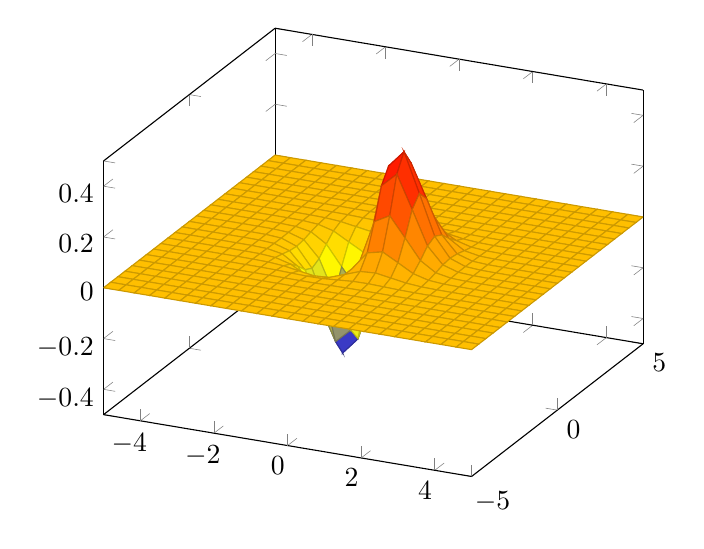
\begin{tikzpicture}
\begin{axis}
\addplot3[
    surf,
]
{exp(-x^2-y^2)*x};
\end{axis}
\end{tikzpicture}

\end{document}
